\begin{figure}
\begin{tikzpicture}
  \node[inner sep=0pt] (circuit) at (0,0) {\includegraphics[scale=2,trim={10mm 0 5mm 0},clip]{Figures/circuits/cnotToCut}};
  \coordinate[left=1mm of circuit.west] (leftPoint);
  \coordinate[right=1mm of circuit.east] (rightPoint);
  \pic (cut) {cut=leftPoint/rightPoint};
  \node[left=-2mm of circuit.north west, font=\itshape] (text) {a)};
  \node[font=\scriptsize\itshape, opacity=0.9, above right=3mm and -4mm of leftPoint] (QPUA) {QPU A};
  \node[font=\scriptsize\itshape, opacity=0.9, below right=3mm and -4mm of leftPoint] (QPUB) {QPU B};
\end{tikzpicture}
\hspace{3mm}
\begin{tikzpicture}
  \node[inner sep=0pt] (circuit) at (0,0) {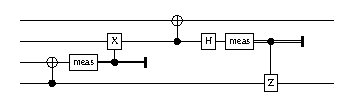
\includegraphics[scale=2]{Figures/circuits/nonlocalCNOT}};
  \pic (e1) {ebit=e1/12.7mm/13mm};
  \coordinate[left=-5.5mm of circuit.west] (leftPoint);
  \coordinate[right=-5.5mm of circuit.east] (rightPoint);
  \pic (cut) {cut=leftPoint/rightPoint};
  \pic [below left=27mm and -13mm of circuit.north west] (entangler) {opaquebox=entangler/9mm/55mm/23mm/41mm/cat-entangler};
  \pic [below left=27mm and -13mm of circuit.north west] (disentangler) {opaquebox=disentangler/9mm/105mm/23mm/39.5mm/cat-disentangler};
  \node[right=2mm of circuit.north west, font=\itshape] (text) {b)};
\end{tikzpicture}
\caption
{A non-local CNOT, shown in \textit{a)}. The dashed line indicates how the circuit is separated into two QPUs. The implementation scheme is given in \textit{b)}.}
\label{fig:nonlocalCNOT}
\end{figure}